%!TEX ROOT=main.tex

\section{LoRa Module Design}
As discussed in section \ref{section:module-architecture}, where the LoRa module was architected and its main parts were selected, the schematic and board layout were created. These outputs are included in image form as Appendix \ref{chapter:module01-files}, along with more details, and available at \link{https://github.com/manakjiri/lora-module-hw/releases/tag/v0.1}{github.com/manakjiri/lora-module-hw}.

The Open source KiCad Electronic Design Automation (EDA) software was used throughout the project to create these designs.

\subsection{\label{section:module-schematic}Schematic}
While the \ref{section:module-architecture} focused on the fundamental parts of the design, many details were left up to the later development stages, once the overall system implementation is more clear. This section will focus and expand on these parts of the design.

Of note is the selection of the main clock source for the MCU \ref{section:mcu}. In this case the only two options are to use a Crystal oscillator (XO) or an Temperature Compensated XO (TCXO). Application note AN5646 (STMicroelectronics \cite{stmicroelectronics_how_nodate-1}) summarizes the main differences as
\begin{itemize}
    \item An XO is more efficient on power consumption, startup time, and BOM cost.
    \item A TCXO is more efficient on frequency accuracy and frequency variation over temperature changes. It also
    removes layout constraints.
\end{itemize}

This aspect was not considered carefully enough during the parts selection, the recommended NX2016SA series crystal oscillator was selected for the power savings and reduced cost. However, the selected programming framework, Embassy, and the library lora--rs in particular (expanded upon in Appendix \ref{chapter:rust}), only correctly supported the use of an TCXO, at the time of the prototype bring--up. This led to an ad hoc modification, documented in Figure \ref{fig:tcxo-bodge}, of the module and the addition of the Abracon ATX--11--F series TCXO to fix this issue.

\begin{figure}
    \centering
    \subfloat[top view]{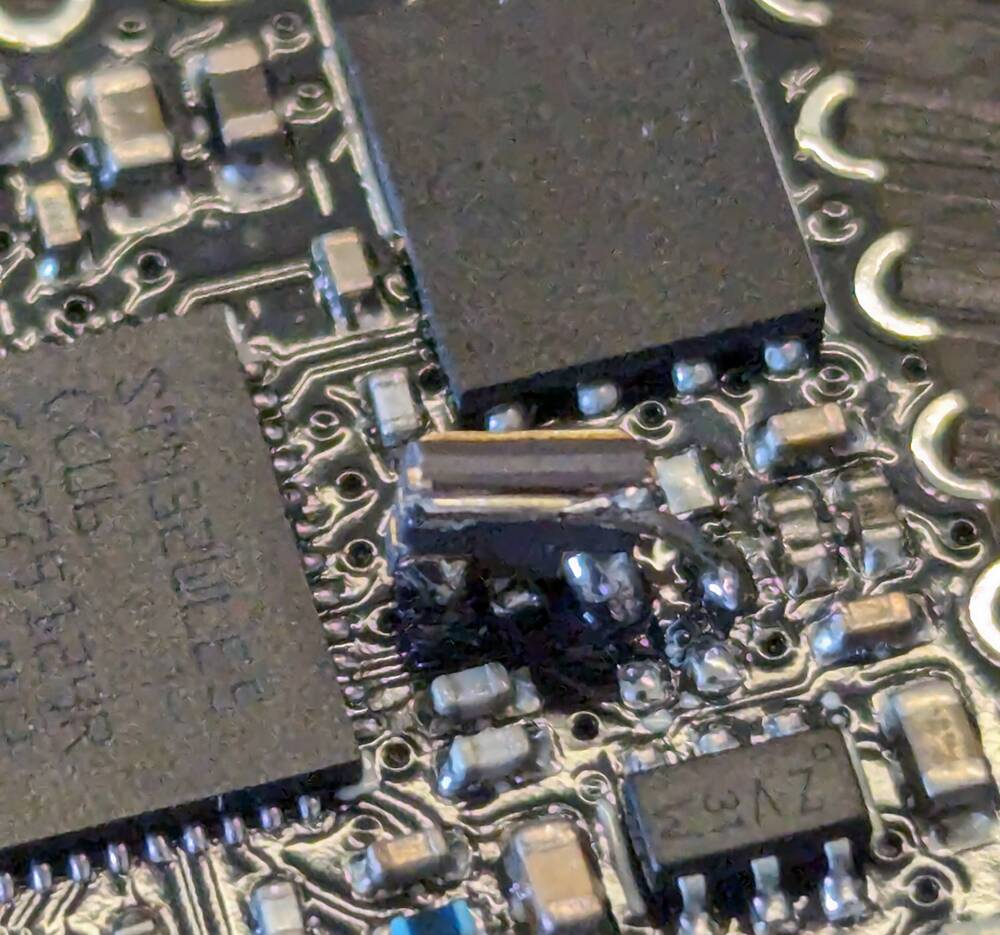
\includegraphics[width=.30\textwidth]{img/tcxo-bodge1.jpg}} \hfil
    \subfloat[side view]{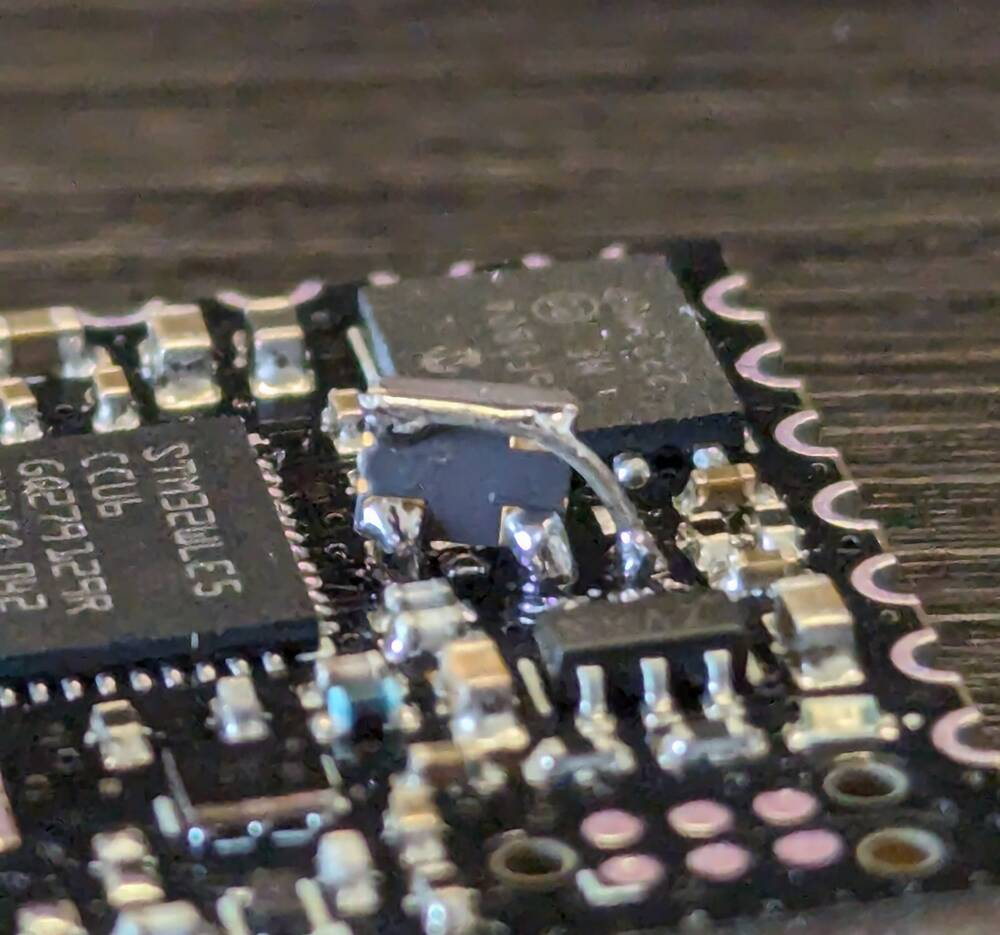
\includegraphics[width=.30\textwidth]{img/tcxo-bodge2.jpg}}
    \caption{\label{fig:tcxo-bodge}The ad hoc TCXO modification on the LoRa module.}
\end{figure}

All other aspects of the MCU integration were executed according to the application notes and the datasheet  \cite{stmicroelectronics_stm32wle5xx_nodate,stmicroelectronics_how_nodate-1}, while closely following the implementations of the reference design and the nucleo development kit \cite{stmicroelectronics_stdes-wl5u4ilh_2024,stmicroelectronics_nucleo-wl55jc_2024}. This includes the selection of decoupling capacitors, the SMPS circuitry and the reset handling.

Another consideration was the implementation of the switchable power rail VDD\_SW. This rail taps off the main power rail of the rest of the module, any disruption could cause a glitch or trigger the BOR protection circuitry. It is thus necessary to limit the inrush current caused by this rail's switch--on and subsequent charging of any local capacitances. An RC circuit was designed to slow--down the gate voltage rise--time to about 10 ms.

\subsection{Printed Circuit Board Layout}
A 4 layer board stackup was proposed in Section \ref{section:mcu}, which indeed ended up being used in this design. Purpose of each layer is described in table \ref{table:board-layers} and clearly observable in the final renders \ref{board:v0.1}.

\begin{table}[H]
\begin{center}
\caption{\label{table:board-layers}Module board layer signal and power assignments.}
    \begin{tabular}{|l|l|} \hline
    \textbf{Layer name}     & \textbf{Primary purpose} \\ \hline
    F. Front layer          & Components and local connections \\ \hline
    1. First inner layer    & Ground \\ \hline
    2. Second inner layer   & Power \\ \hline
    B. Back layer           & Signal and markings \\ \hline
    \end{tabular}
\end{center}
\end{table}

The board is only populated on the front side, see Figure \ref{board:v0.1-components}, to allow its use as a solder--able module. Still, the final dimensions of the module are $20.32 \times 22.48~\mathrm{mm}$, which is better than the initial optimistic estimate given in Section \ref{section:antenna}.

To stay compatible with low--cost manufacturing options, conservative parameters were picked when it comes to minimal clearance, trace width and drill size. No density--increasing technologies, such as blind or buried vias, via--in--pad, micro--via, etc. were employed either. 

These parameters are summarized in the following Table \ref{table:board-limits} and were enforced by the Design Rule Checker (DRC) throughout the project.

\begin{table}[H]
\begin{center}
\caption{\label{table:board-limits}Board layout physical limits.}
    \begin{tabular}{|l|l|} \hline
    \textbf{Parameter}          & \textbf{Dimension} \\ \hline
    Minimum trace clearance & $0.15~\mathrm{mm}$ \\ \hline
    Minimum trace width & $0.15~\mathrm{mm}$ \\ \hline
    Minimum via width & $0.3~\mathrm{mm}$ \\ \hline
    Hole to trace clearance & $0.3~\mathrm{mm}$ \\ \hline
    Hole to hole clearance & $0.5~\mathrm{mm}$ \\ \hline
    Board edge to trace clearance & $0.15~\mathrm{mm}$ \\ \hline
    \end{tabular}
\end{center}
\end{table}

Being only 4 layers, the traces needed to be routed in densely and well thought--out manner, attempting to minimize the number of relatively large vias required. For this reason, the module's external connection signal assignments were decided only near the end of the design stage conforming mostly to the existing pin locations on the MCU itself. The final pad assignments are included in Table \ref{table:module-pin-legend}.

\begin{figure}
    \includesvg[width=.75\textwidth]{img/module-v0.1.drawio.svg}
    \caption{\label{fig:module-v0.1}Image of the manufactured and fully assembled module with overlay highlighting its functional parts.}
\end{figure}

\subsection{Finalized LoRa Module Specification}
Figure \ref{fig:module-v0.1} shows the manufactured and fully assembled module with overlay highlighting its functional parts, its technical specifications are captured by Table \ref{table:module-specification}.

\begin{table}[p]
\begin{center}
\caption{\label{table:module-specification}Final module specification.}
    \begin{tabular}{|l|l|} \hline
    Supply voltage range                    & $2.3\text{--}3.5~\mathrm{V}$\\ \hline
    Maximum supply current (excluding EXT)  & $65~\mathrm{mA}$\\ \hline
    %Standby supply current                  & $10--500~\mathrm{uA}$\\ \hline
    Operating temperature range             & $-40\text{--}85~\mathrm{^\circ C}$\\ \hline
    Output RF power                         & $15~\mathrm{dBm}$\\ \hline
    Operating band                          & $868~\mathrm{MHz}$\\ \hline
    RF connector                            & U.FL \\ \hline
    Module connection type                  & Castellated hole (0.1 inch pitch) \\ \hline
    Supported interfaces                    & UART, SPI, I2C \\ \hline
    Programming interface                   & ARM Serial Wire Debug (SWD) \\ \hline
    \end{tabular}
\end{center}
\end{table}

\begin{table}[p]
\begin{center}
\caption{\label{table:module-pin-legend}Module pin legend including feature summary.}
    \begin{tabular}{|l|l|l|l|l|l|l|l|l|} \hline
    \textbf{IO} & \textbf{Pin} & \textbf{TIM\footnote{Refer to each column following ``Pin'' (excluding ``Other'') as [Column header][Column-row contents], such as ``SPI1\_MOSI'' and so on. Some features were omitted for clarity, for complete list refer to the MCU manufacturer's documentation}} & \textbf{ADC} & \textbf{I2C} & \textbf{SPI} & \textbf{UART} & \textbf{Other}\\ \hline
    1  & PA7  & 17\_1, 1\_1N    &     & 3\_SCL & 1\_MOSI &             & CMP2\_OUT          \\ \hline
    2  & PA6  & 16\_1          &     &       & 1\_MISO &             &                    \\ \hline
    3  & PA4  & L1,2\_OUT      &     &       &        &             & RTC\_OUT2           \\ \hline
    4  & PA2  & 2\_3           &     &       &        & 2\_TX      & CMP2\_OUT           \\ \hline
    5  & PA1  & L3\_OUT, 2\_2   &     &       & 1\_SCK  &             &                    \\ \hline
    6  & PA0  & 2\_1           &     &       &        &             & WKUP1   \\ \hline
    7  & PB8  & 16\_1, 1\_2N    &     & 1\_SCL &        &             &                    \\ \hline
    8  & PB7  & L1\_IN2, 17\_1N &     & 1\_SDA &        & 1\_RX        &                    \\ \hline
    9  & PB6  &               &     & 1\_SCL &        & 1\_TX        &                    \\ \hline
    10 & PB5  & L1\_IN1        &     &       & 1\_MOSI &             & CMP2\_OUT          \\ \hline
    11 & PB4  &               & 3   & 3\_SDA & 1\_MISO &             & CMP1,2\_INP        \\ \hline
    12 & PA11 & 1\_4           & 7   & 2\_SDA & 1\_MISO &             & CMP1,2\_INM        \\ \hline
    13 & PB3  & 2\_CH2         & 2   &       & 1\_SCK  &             & SWO, WKUP3 \\ \hline
    14 & PA13 &               & 9   &       &        &             & SWDIO            \\ \hline
    15 & PA14 & L1\_OUT        & 10  &       &        &             & SWCLK                   \\ \hline
    16 & PH3  &               &     &       &        &             & BOOT0                   \\ \hline
    \end{tabular}
\end{center}
\end{table}

\subsection{Radio Performance}
The output RF characteristics were validated using a spectrum analyzer connected directly to the RF output of the module through an U.FL pigtail.

The module was setup in ``continuous wave'' mode \cite{semtech_corporation_sx12612_2024} at 869.525 MHz with power of 15 dBm, which produced the spectrogram visible in Figure \ref{fig:rf-mask-wave}. Here we can observe, that the peak power was measured at 12.60 dBm and the frequency is off by 150 kHz.

\begin{figure}
    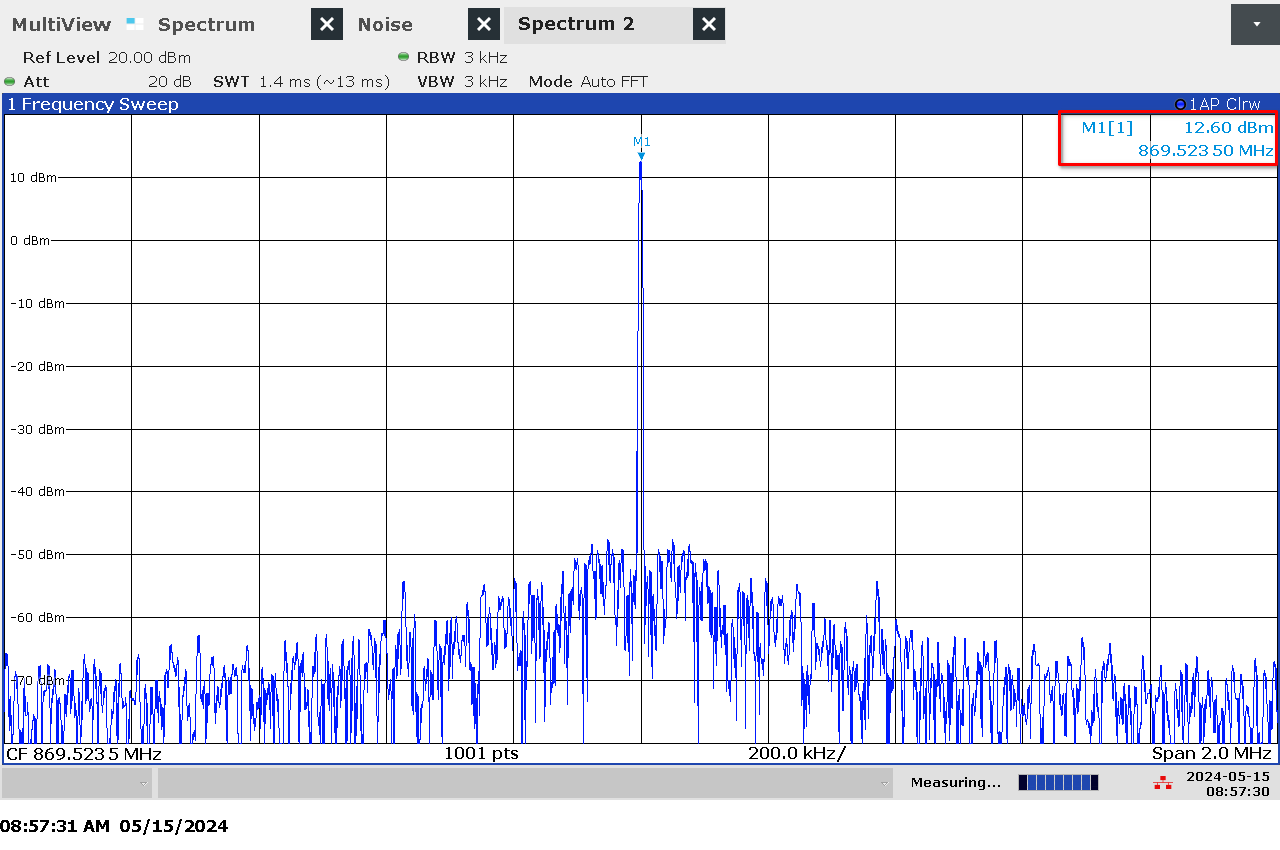
\includegraphics[width=.9\textwidth]{fig/rf-mask-wave.png}
    \caption{\label{fig:rf-mask-wave}Measurement of the module RF output in ``continuous wave'' mode at 869.525 MHz with power of 15 dBm}
\end{figure}

Next two measurements in Figure \ref{fig:rf-power}, are captures of the module transmitting 8 bytes of data at SF5, bandwidth 250 kHz and coding rate 4:5, the rest of the parameters is identical as in Table \ref{table:range-test-parameters}. 

These measurements show that the output power stays stable at 13 dBm once modulating and that there are smooth transitions and power ramp up, suggesting good power supply and power management design. The mask visible in the spectrum is uniform, without any unexpected artifacts.

\begin{figure}[p]
    \centering
    \subfloat[Spectogram of the transmitted signal (upper), waterfall graph of the spectrum (lower)]{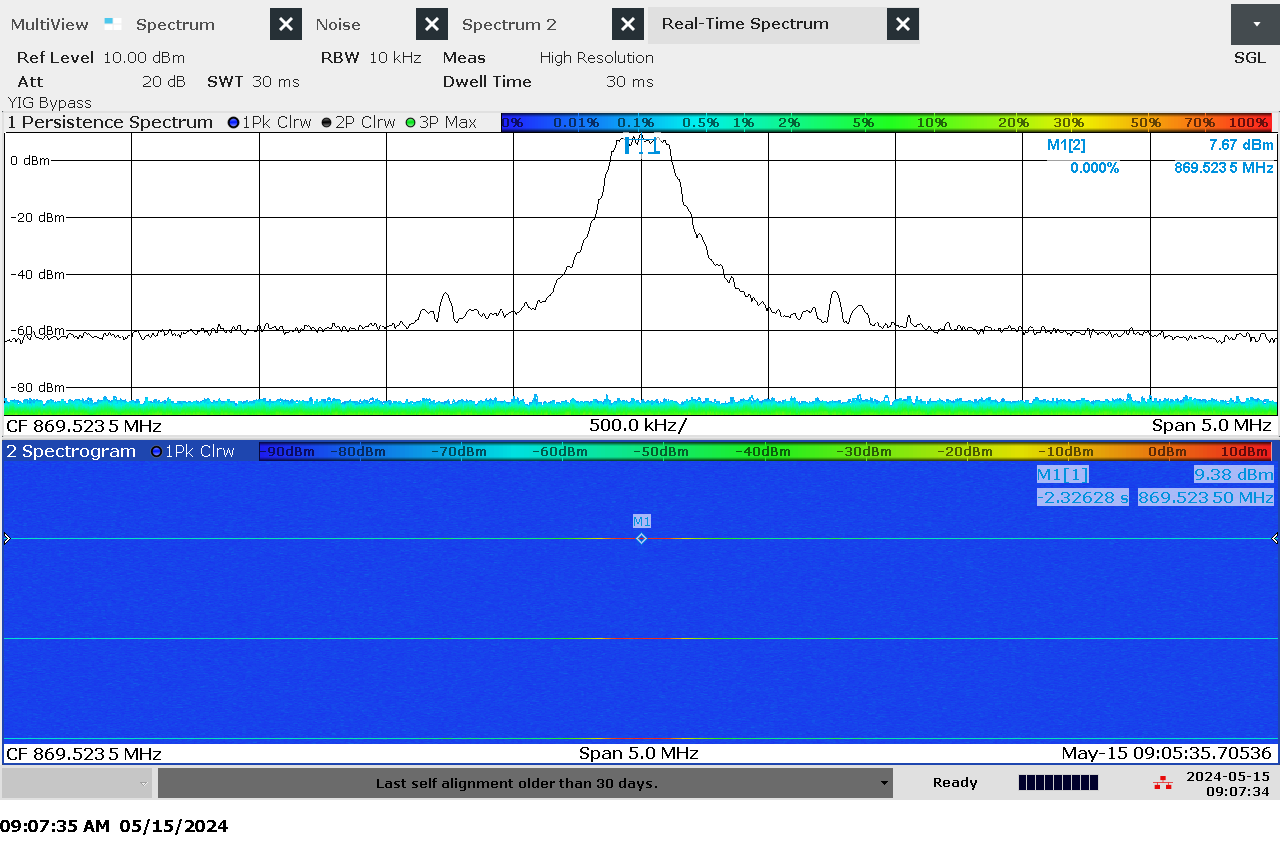
\includegraphics[width=.9\textwidth]{fig/rf-transmit-250khz.png}} \hfil
    \subfloat[Packet in the time domain (upper), Packet spectrum (lower)]{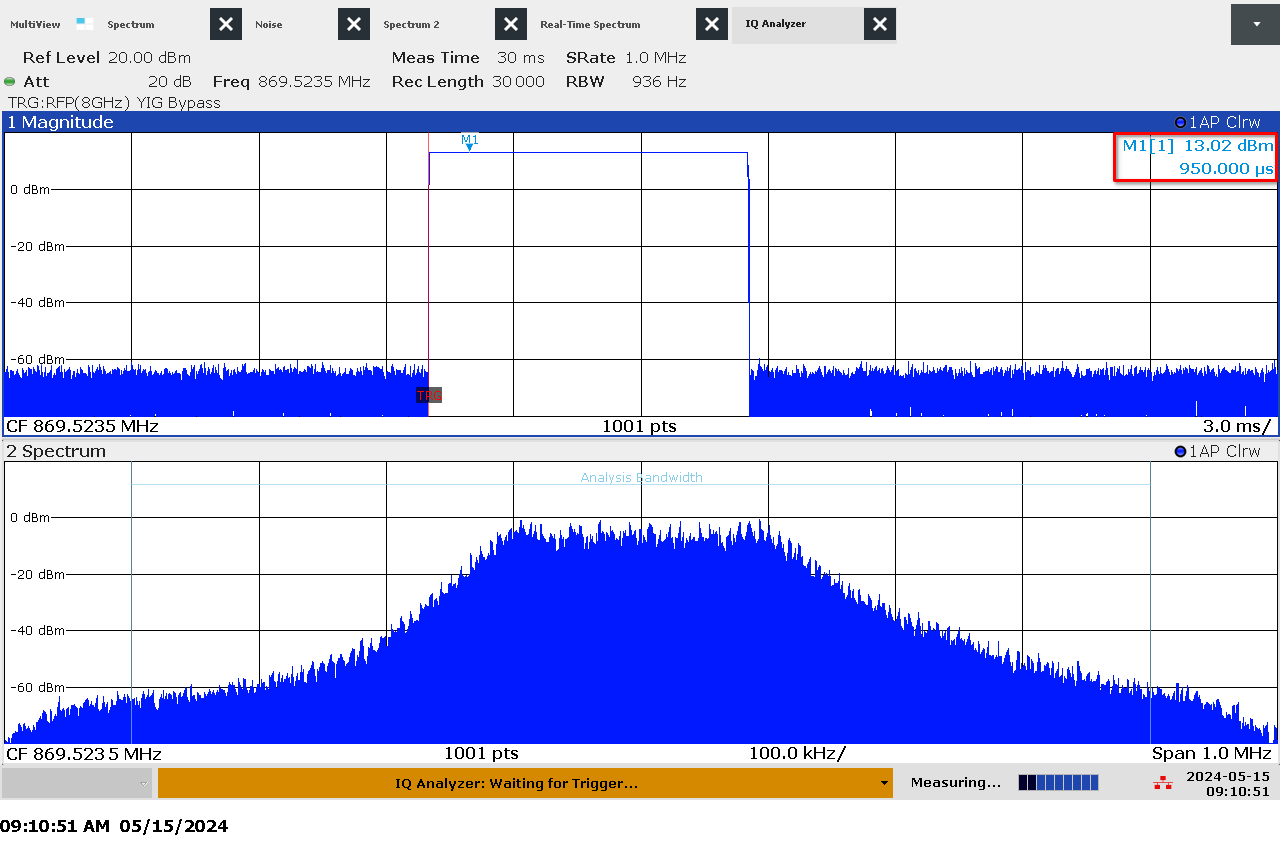
\includegraphics[width=.9\textwidth]{fig/rf-power.png}}
    \caption{\label{fig:rf-power}Capture of the module transmitting 8 bytes of data at SF5, bandwidth 250 kHz and coding rate 4:5, the rest of the parameters is identical as in Table \ref{table:range-test-parameters}}
\end{figure}

\subsection{Power Consumption}
Because of the improvised replacement of the crystal oscillator with a TCXO, which exhibits much higher power consumption (2--3 mA) and an inability to connect its power supply to the pin PB0, which is designed to power this oscillator and gate its power supply whenever it is not needed, the module exhibits higher than expected power draw of around 9 mA while receiving and 6 mA while idle. The fix is documented in Section \ref{section:module-v0.2}.

\begin{figure}
    \centering
    \subfloat[Continuous receive with transmit in the middle]{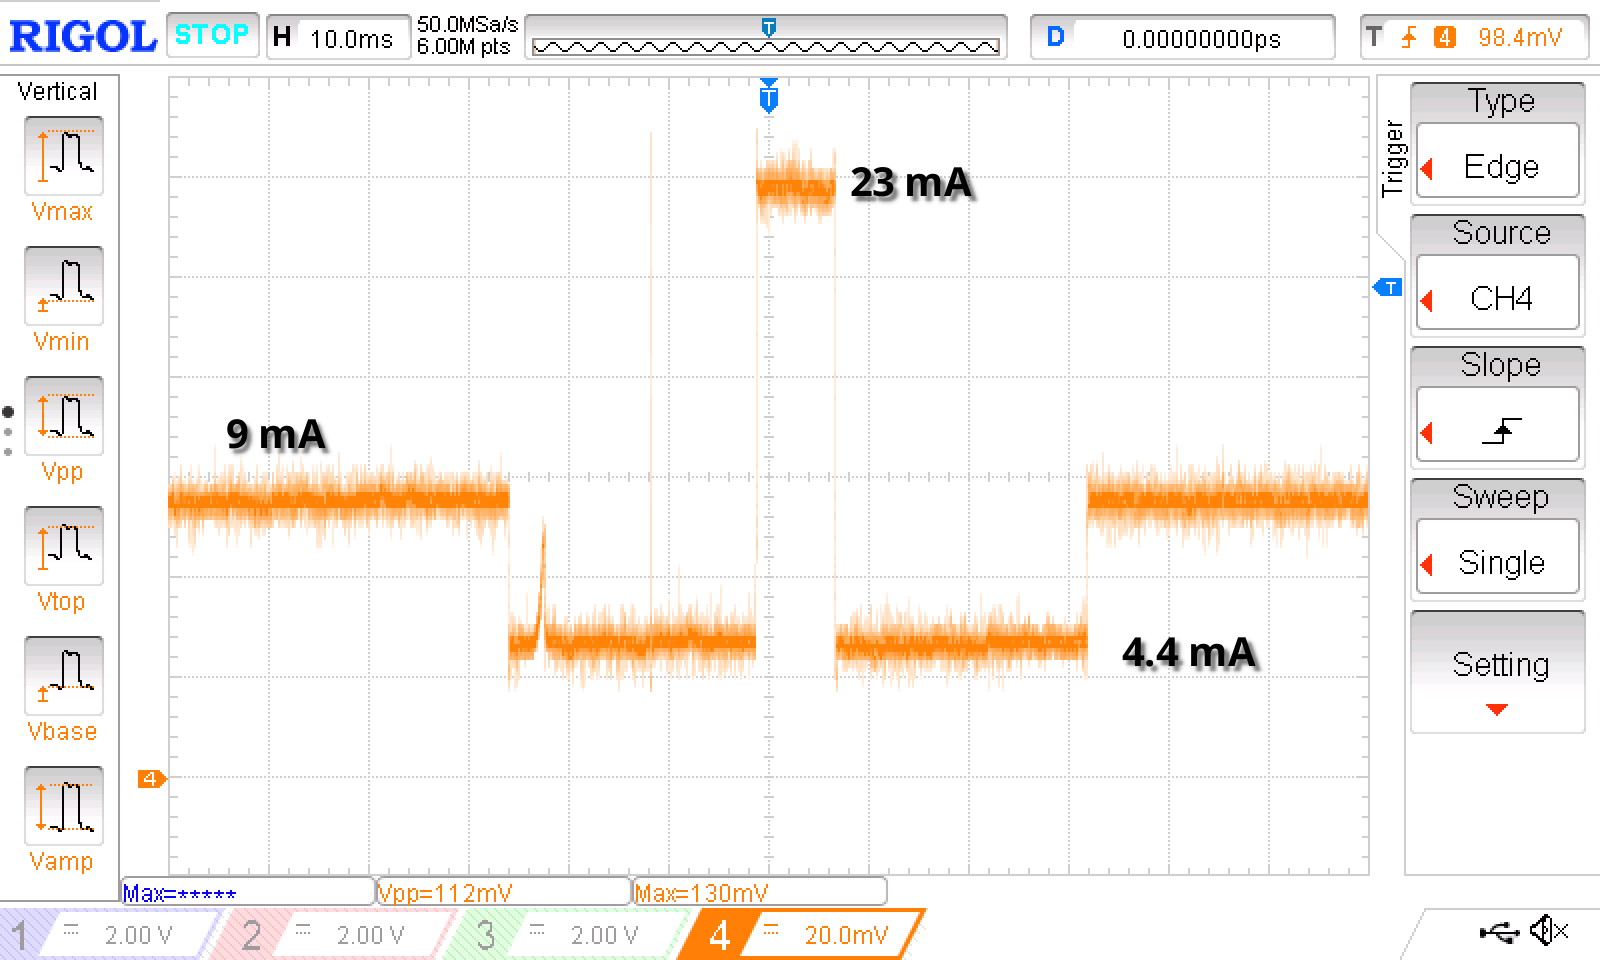
\includegraphics[width=.49\textwidth]{fig/module-current-rx-inv.png}} \hfil
    \subfloat[Idle, transmit, receive acknowledge]{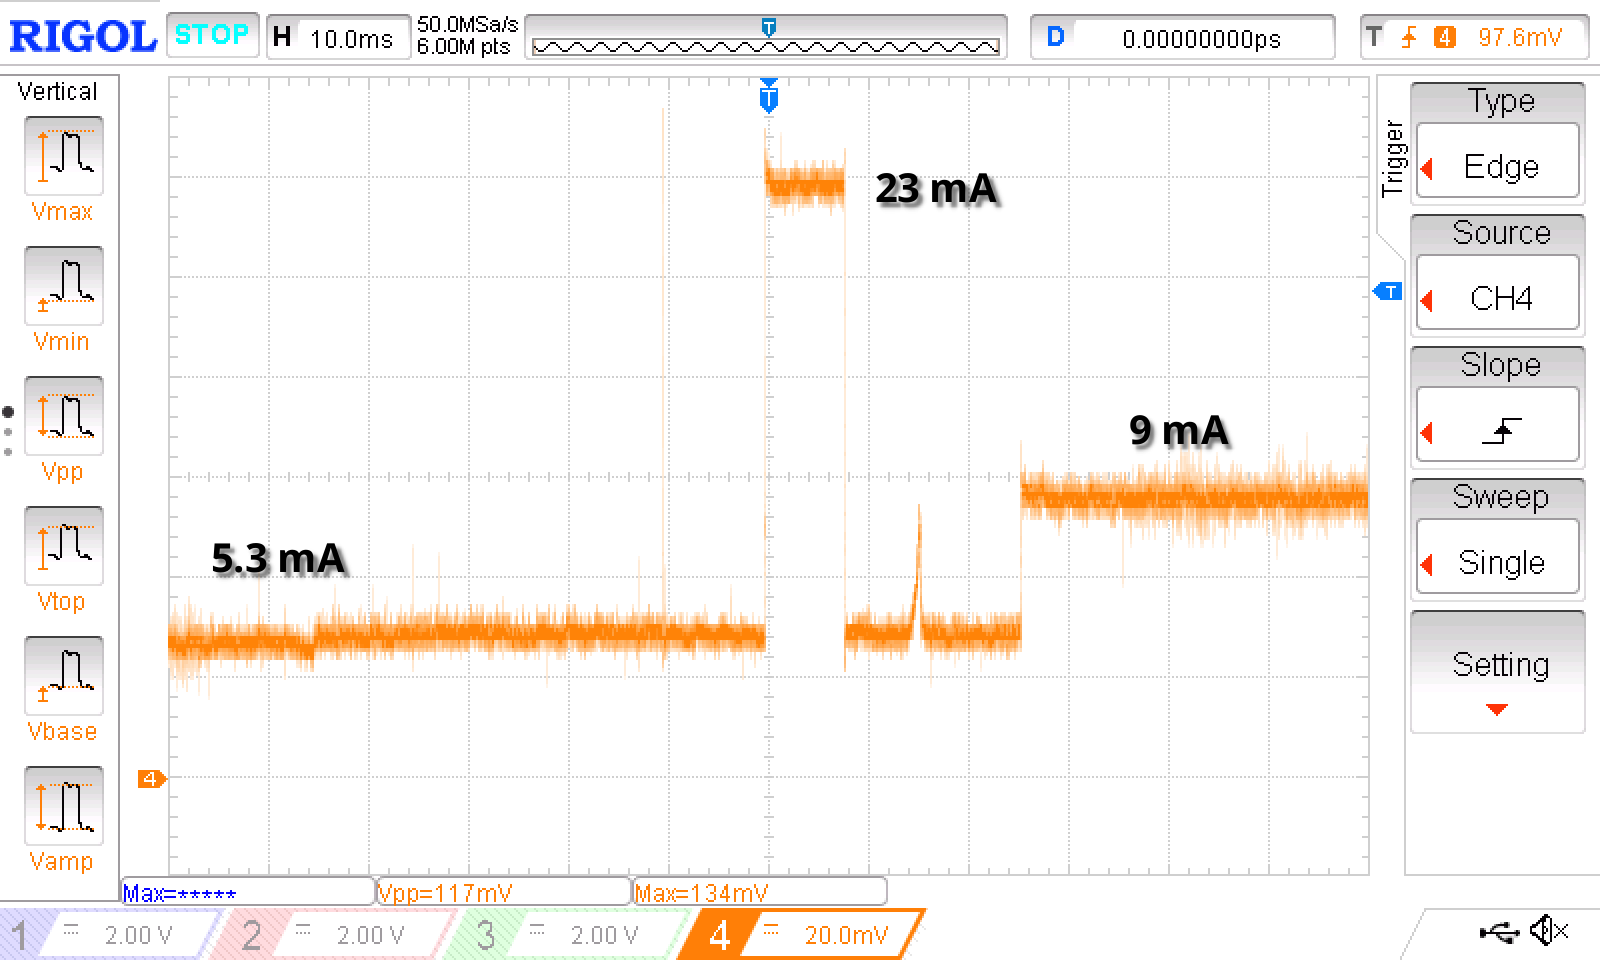
\includegraphics[width=.49\textwidth]{fig/module-current-tx-inv.png}}
    \caption{\label{fig:module-current}Current waveform of the module measured through a 5.6 $\Omega$ resistor in different operational scenarios.}
\end{figure}

The idle power draw could be optimized to reach 10--100s of $\mu$A with the TCXO properly connected and significant time investment into the firmware development. The current consumption waveform can be examined in Figure \ref{fig:module-current}.

\section{Soil Moisture Sensor Design}
\begin{figure}[H]
    \includesvg[width=\textwidth]{boards/sensor/soil-sensor-F_Cu.svg}
    \caption{\label{fig:sensor-pcb}Printed Circuit Board design of the top layer of the soil moisture sensor board, where the 4 capacitive sensing zones are distinctly visible. These capacitors form, what is later referred to, as the ``active area'' of the sensor. More is available in Appendix \ref{chapter:sensor-files}.}
\end{figure}
To summarize, the soil moisture sensor board contains
\begin{itemize}
    \item the capacitance measuring circuit (as described in Section \ref{section:measuring-method}) with two ranges,
    \item a dual single pole quadruple throw (Dual SP4T) mux chip for switching between the 4 sensing zones contained in the active area of the sensor,
    \item 8 channel TVS diode array to clamp the voltage on the capacitor electrodes and means of isolating the sensor elements from the measuring circuits,
    \item a 2.8 V linear low-dropout (LDO) regulator,
    \item footprint for the LoRa module,
    \item two analog temperature sensor ICs and
    \item single cell rechargeable lithium battery protection circuitry.
\end{itemize}

\subsection{\label{section:sensor-circuit}Capacitance Measuring Circuit}
Of note is the performance of the capacitance measuring circuit, which was validated using an oscilloscope connected to the test-points on the sensor board, see Figure \ref{fig:cap-measure}.
\begin{figure}[H]
    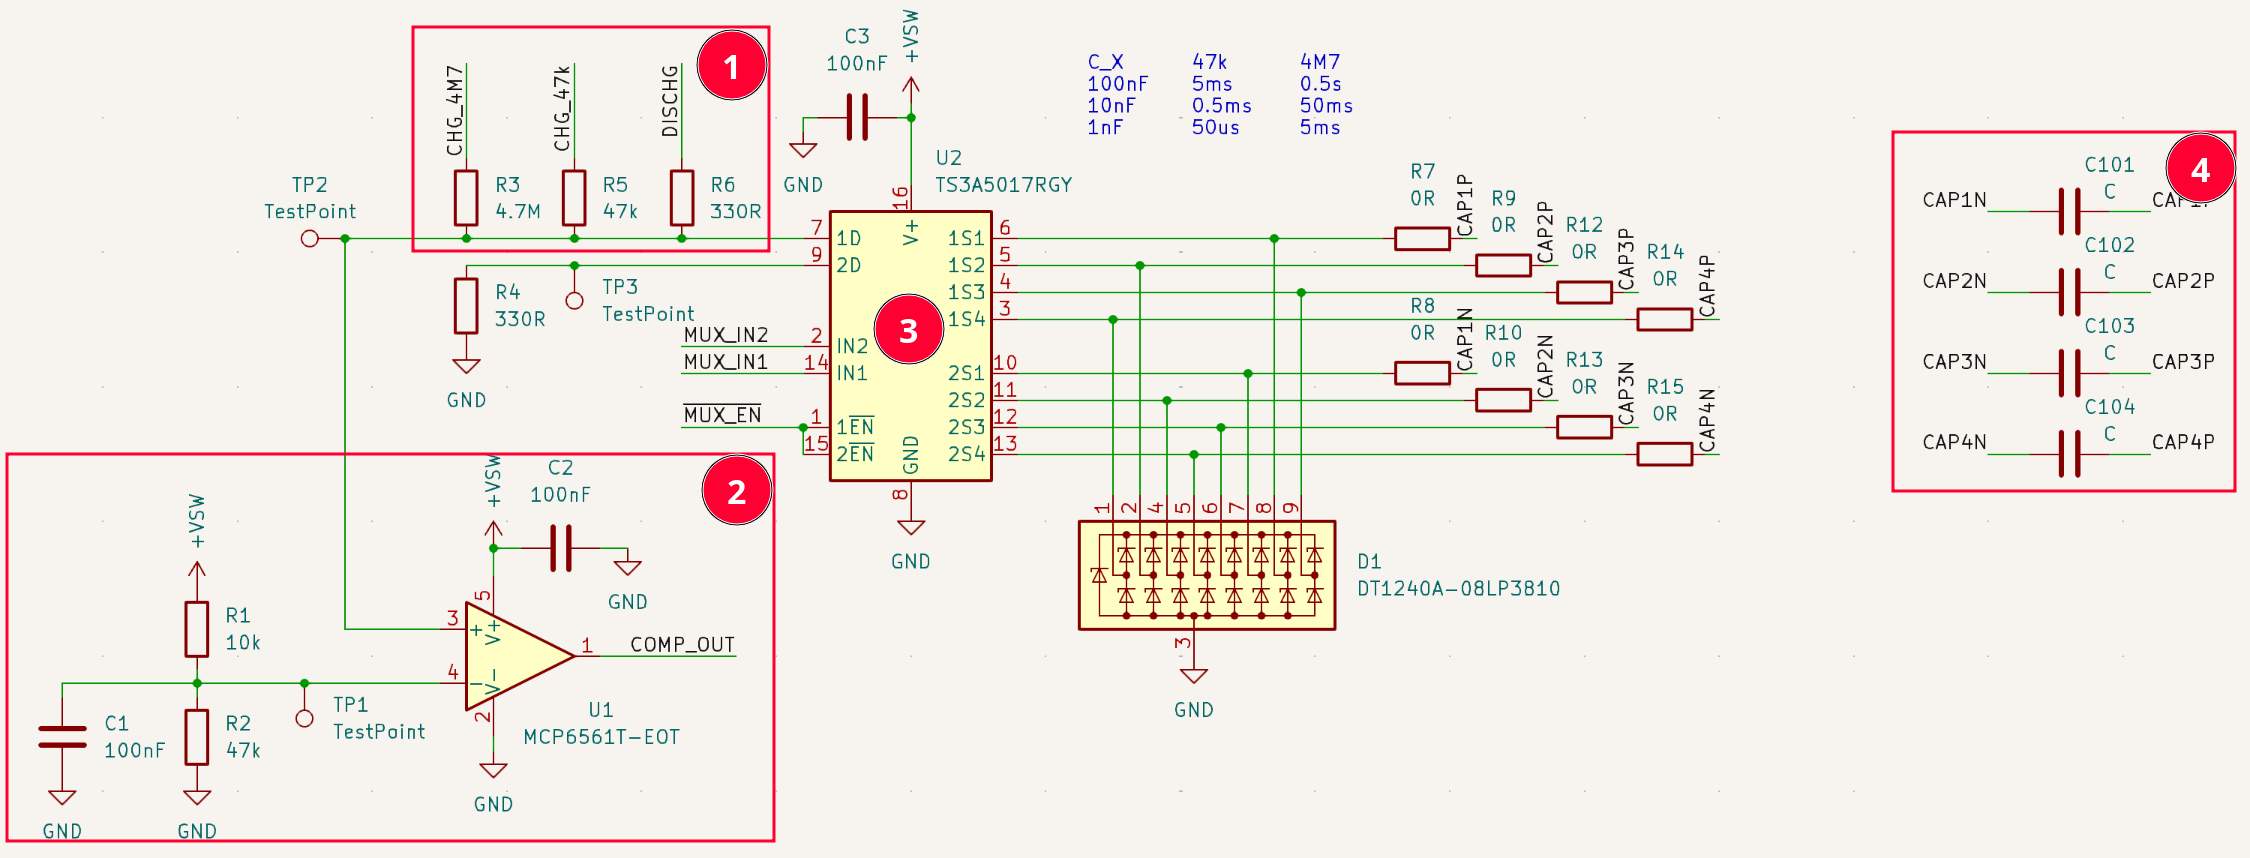
\includegraphics[width=.9\textwidth]{fig/sensor-measure-circuit.png}
    \caption{\label{fig:sensor-measure-circuit}The capacitance measuring circuit functions by charging the unknown capacitor $C_X$ through a known resistor $R_{CHG}$ and measuring the time it takes to reach a certain voltage derived from a voltage reference. The muxing (U2) and protection circuitry (D1) is also included. Resistors R7--15 are there to facilitate a complete isolation of the sensor from the measuring circuit, for measuring the capacitor elements externally, if the need be, without damaging the board. The full schematic is available in Appendix \ref{chapter:sensor-files}.}
\end{figure}

The capacitance can be calculated from readings obtained in Figure \ref{fig:cap-measure}. Given the charging voltage $U = 3.3~\mathrm{V}$ (it may not seem so from the Figure, due to the charging resistor being disconnected as soon as the threshold voltage is reached). The capacitance RC time constant is defined as
\begin{equation} %(7.6*10^-6)/(47*10^3)
    \tau = RC ~~~\rightarrow~~~ C = \dfrac{\tau}{R} = \dfrac{7.6 \cdot 10^{-6}}{47 \cdot 10^3} = 161~\mathrm{pF}.
\end{equation}
This result goes in line with the estimate given in Section \ref{section:expected-cap}. The reading would triple when submerged fully in water.

\begin{figure}[H]
    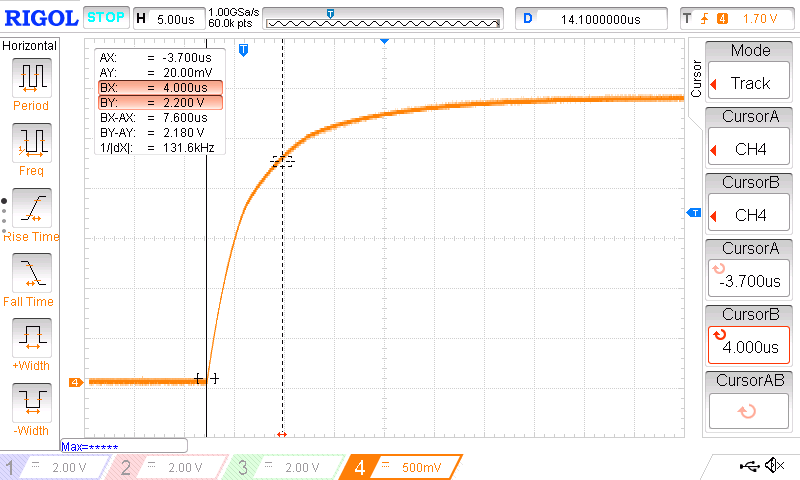
\includegraphics[width=.8\textwidth]{fig/cap-measure-inv.png}
    \caption{\label{fig:cap-measure}Sensor capacitor (in air) voltage rise time measurement when charged through a 47k$\Omega$ resistor, which was later replaced by a different value to increase the measuring time.}
\end{figure}

The original 47 k$\Omega$ and 4.7 M$\Omega$ resistors were replaced by 100 k$\Omega$ and 1 M$\Omega$ resistors to improve the measuring performance. These resistors were designed with this possibility in mind and a larger footprint was used to make this process easier. the 4.7 M$\Omega$ resistor was not able to charge the circuit up to the detecting threshold of the comparator, because the rest of the components incurred parasitic resistance to ground of about 15 M$\Omega$, forming a voltage divider.

This setup provides repeatable and stable measurements in free air and when the capacitor is completely submerged in water. It is sensitive enough to reliably detect close proximity (1 cm) or touch of a human hand.

The following code is responsible for each sample conversion, refer to the comments for principle explanation.
\newpage
\begin{lstlisting}
pub async fn sample_current_channel(
        &mut self, range: SoilSensorRange
    ) -> SoilSensorResult {
    /* 1. Handle the range selection by setting the required charge 
    pin as output and the unused pin as high-impedance input. */
    match range {
        SoilSensorRange::Low => {
            self.chg_1m.set_as_input(Pull::None);
            self.chg_100k.set_as_output(Speed::Low);
            self.chg_100k.set_low();
        },
        SoilSensorRange::High => {
            self.chg_100k.set_as_input(Pull::None);
            self.chg_1m.set_as_output(Speed::Low);
            self.chg_1m.set_low();
        },
    }
    /* 2. Bridge the connection between the selected capacitor 
    and the rest of the measuring circuit (the channel selection 
    happens before this function) and discharge the capacitor. */
    self.dischg.set_low();
    self.mux_nen.set_low();
    Timer::after_micros(100).await;
    /* Note: the DISCH pin is configured as open-drain output. */
    self.dischg.set_high();
    /* 3. Start charging the capacitor through the selected resistor. */
    match range {
        SoilSensorRange::Low => {
            self.chg_100k.set_high();
        },
        SoilSensorRange::High => {
            self.chg_1m.set_high();
        },
    }
    let start = Instant::now();
    /* 4. Await either the interrupt from the COMParator input
    or a timeout in case a wrong range was selected. */
    let ret = match select(
        self.comp.wait_for_high(), 
        Timer::after_millis(2)
    ).await {
        Either::First(_) => {
            /* 5a. Calculate the measured time to be returned 
            in case of successful conversion */
            let mut elapsed = start.elapsed();
            match range {
                SoilSensorRange::Low => {
                    elapsed *= 10;
                },
                SoilSensorRange::High => {
                    elapsed *= 1;
                },
            }
            SoilSensorResult::Ok(elapsed.as_micros() as u16)
        },
        /* 5b. Timeout */
        Either::Second(_) => SoilSensorResult::Timeout,
    };
    /* 6. Return all pins to default state */
    self.chg_100k.set_as_input(Pull::None);
    self.chg_1m.set_as_input(Pull::None);
    self.dischg.set_low();
    self.mux_nen.set_high();
    ret
}
\end{lstlisting}

\FloatBarrier
\section{\label{section:ota-implementation}Over--the--air Update Implementation}
It is the responsibility of the update process to securely and reliably transfer the binary image of the firmware from the host computer through the Gateway to the designated Node (sensor) of the network. 

This task is complicated by the limited resources available on embedded devices, as discussed in Section \ref{section:ota-update-support}, and the slow and sometimes unreliable nature of the wireless connection in general. Following sections describe the protocol solution to this aspect of the OTA update process.

The performance testing was done along with the range test described in the following Section \ref{section:range-test}.

\subsection{Data Fragmentation}
The binary needs to be fragmented in order to be transmitted piece by piece. To guarantee the assembly of these fragments on the Node, an acknowledge mechanism must be present along with a way to detect errors in the transferred data. While the LoRa physical layer provides forward error correction and also up to a 16 bit CRC checksum, the error rate is from experience still too high to be practical. To tackle this, a custom 32 bit CRC was used to protect each fragment together with a SHA256 hash of the whole assembled binary, which is calculated as the last step in the update process.

\begin{figure}[p]
    \includesvg[width=0.9\textwidth]{fig/ota-algo.drawio.svg}
    \caption{\label{fig:ota-algo}Simplified flowchart depicting the over--the--air update communication process between the Gateway and the Node.}
\end{figure}

Figure \ref{fig:ota-algo} provides a basic overview of the OTA update process. The communication with the host is left out for brevity, but mostly mirrors the operations that happen on the Gateway. Names in the cells correspond to packet types defined in the \link{https://github.com/manakjiri/lora-module-fw/blob/main/module-runtime/src/ota/common.rs}{module-runtime/src/ota/common.rs} file as \code{enum OtaPacket}. Packets are serialized and deserialized using the \link{https://docs.rs/postcard/latest/postcard/}{postcard} Rust package.

\subsection{Acknowledge Mechanism}
The Automatic Repeat Request (ARQ) mechanism is inspired by Selective Repeat ARQ. The receiver is able to accept frames that are out of order and selectively requests missing or corrupted blocks. In contrast to standard ARQ, here the acknowledge (ACK) packet contains up to 32 indexes of blocks that were successfully received, instead of just one.

Likewise, the transmitter does not expect to receive ACK packets consistently and continues to transmit in order for up to 16 unACKed frames. The receiver is thus able to relax the rate of ACK packets to reduce the air time usage. Since the transmitter is not attempting to use the maximum available channel capacity, it transmits about one packet per second, it does not need the immediate response to measure latency.

\subsection{Bootloader}
Once the data was transferred to the target Node to be updated, the Node needs to perform the update by swapping the old firmware image with the new one, as described in Section \ref{section:ota-update-support}. The Embassy Bootloader was used for this purpose, as it is easy to integrate, features small memory footprint of just 8 KBytes, along with a rollback feature \cite{embassy_project_documentation_bootloader_2024}. The rollback is initiated after device reset if the application failed to signal to the bootloader, that it started up successfully by writing a special value in the state section of the FLASH.
